% \section{数学工具}
% \subsection{拉普拉斯分布}
% % 合成图像数据集往往假设低分辨率图像由高分辨率图像经高斯模糊和双三次下采样得到,使用公式表示即为:
% % \begin{equation}
% %     \mathbi{I}^{LR}=(\vb*{k}_g\otimes \mathbi{I}^{HR})\downarrow_s
% % \end{equation}
% 拉普拉斯分布是以法国数学家Pierre-Simon命名的一种连续概率分布,又称双指数分布。拉普拉斯分布的概率密度函数为
% \begin{equation}
%     f(x;\mu, b)=\frac{1}{2b}\exp(-\frac{|x-\mu|}{b})
% \end{equation}
% 其中,$\mu$为位置参数,表示其对称轴位置;$b$为尺度参数,表示其开口尺度。其概率密度函数与累计分布函数如图\ref{fig:laplace-a}\ref{fig:laplace-b}所示。在本文所基于的模型USR-DU中,作者经过实验发现真实的低分辨率图像与双三次下采样图像之间的差异呈拉普拉斯分布,如图\ref{fig:laplace-c}所示。
% \begin{figure}[h]
%     \subcaptionbox{\label{fig:laplace-a}}{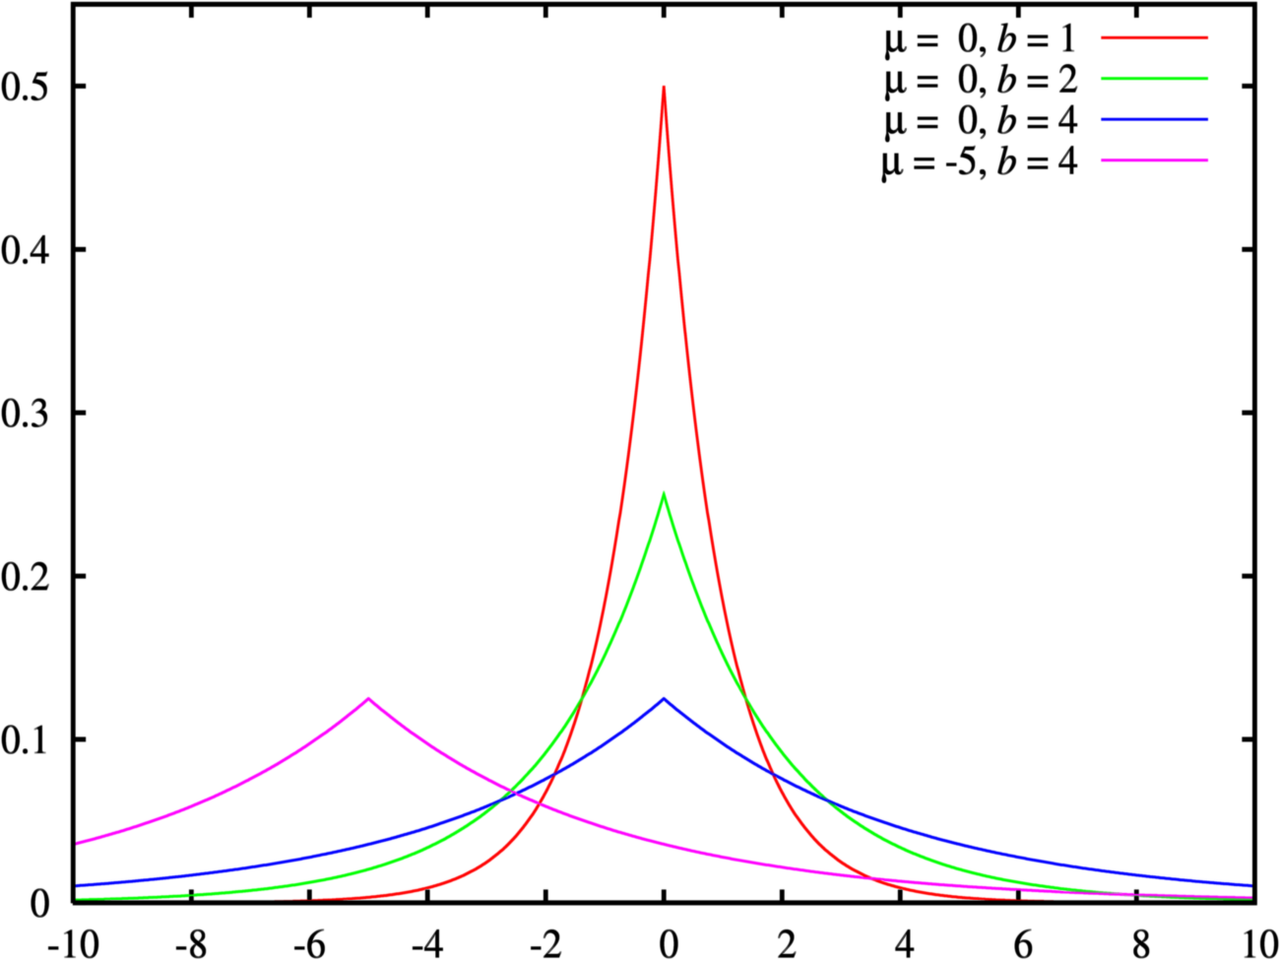
\includegraphics[width=.3\linewidth]{imgs/laplace_wiki_1.png}}\hfill
%     \subcaptionbox{\label{fig:laplace-b}}{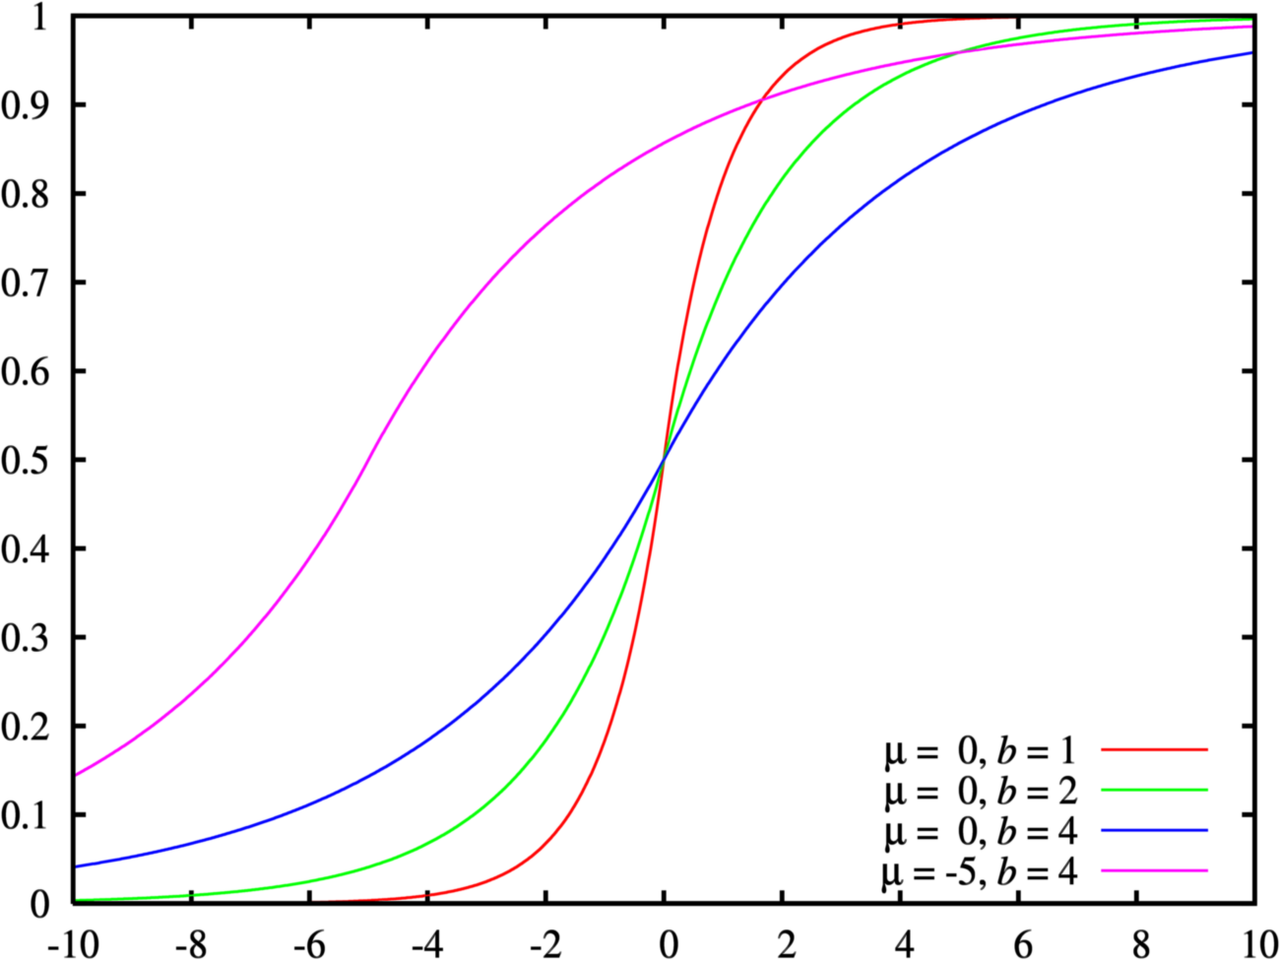
\includegraphics[width=.3\linewidth]{imgs/laplace_wiki_2.png}}\hfill
%     \subcaptionbox{\label{fig:laplace-c}}{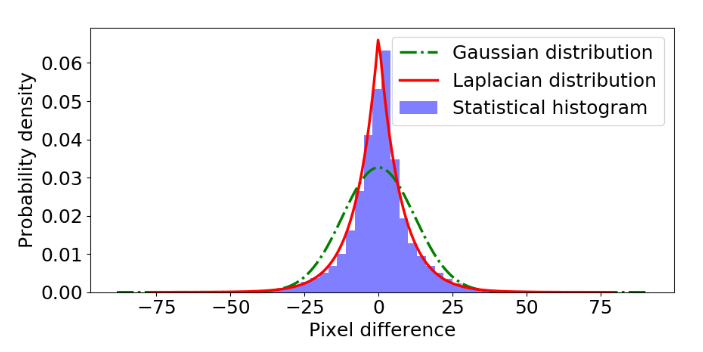
\includegraphics[width=.4\linewidth]{imgs/laplace_usr-du.png}}
%     \caption{拉普拉斯分布:其中,图(a)为概率密度函数,图(b)为累计分布函数,图(c)为USR-DU论文中作者对真实低分辨率图像与双三次下采样图像间差异分布进行实验的结果,作者发现实际的分布近似于拉普拉斯分布而不近似于高斯分布}	
%     \label{fig:laplace}
% \end{figure}

% \subsection{KL散度}
% KL散度(Kullback-Leibler divergence)又称相对熵,描述了$P$,$Q$两个分布之间的差异,其中$P$为真实分布,$Q$为估计分布。对于连续随机变量,KL散度可定义为
% \begin{equation}
%     D_{\text{KL}}(P\|Q)=\int^\infty_{-\infty}p(x)\ln\frac{p(x)}{q(x)}\,\text{d}x
% \end{equation}

% 在USR-DU中,DSN输出低分辨率图像$\vb*{y}_g$及其不确定性$\bm{\theta}$,其实质为输出了估计的低分辨率图像的分布。故为了优化网络,使其估计出正确的分布,可使用KL散度来构造损失函数
% \begin{equation}
%     \begin{aligned}
%         \mathcal{L}_{kl}&=\mathbb{E}_{\vb*{y}_g}\{D_{\text{KL}}[L(\vb*{y}_g,\bm{\theta})\|L(\vb*{y}_b,\mathbi{I})]\}  \\
%         &=\mathbb{E}_{\vb*{y}_g}[\bm{\theta}\exp(-\frac{\|\vb*{y}_g-\vb*{y}_b\|_1}{\bm{\theta}})+\|\vb*{y}_g-\vb*{y}_b\|_1-\ln\bm{\theta}-1]
%     \end{aligned}
%     \label{equ:kl}
% \end{equation}
% 其中$\vb*{y}_b$为双三次下采样图像,$\mathbi{I}$为单位矩阵。


% \section{超分辨率模型的评价指标}
% 为了能够评判各种超分辨率模型间精度的优劣,需要采用多种指标进行评价。而不同的评价指标则拥有不同的侧重点。
% \subsection{基于参考的评价指标}
% 此类指标是最常用的评价指标。其中,PSNR(Peak Signal-to-Noise Ratio,峰值信噪比)通过比较原始图像与经过处理后的图像的信噪比来衡量两张图像之间的差距,单位为分贝(dB),取值范围为0到无穷大。PSNR越大,则说明两张图像越相近。PSNR的定义式为:
% \begin{equation}
%     \text{PSNR}=10\cdot \log_{10}(\frac{\text{MAX}_I^2}{\text{MSE}})
% \end{equation}
% 其中,$MAX_I$是像素的最大值,这取决于像素值是$0\sim 255$还是$0\sim 1$;MSE(Mean Square Erros)是两张图像之间的均方误差。

% SSIM\cite{wang2002universal}(Structural Similarity Index Measure,结构相似性指标)除了考虑除了像PSNR考虑像素间差异以外,还考虑图像的结构、纹理、对比度等因素。SSIM没有单位,取值范围为-1到1,SSIM越大,说明两张图像相似度越高。SSIM的定义为
% \begin{equation}
%     \begin{aligned}
%         SSIM(x,y)&=[l(x,y)s(x,y)c(x,y)]
%                  &=\frac{(2\mu_x\mu_y+c_1)(2\sigma_{xy}+c_2)}{(\mu_x^2\mu_y^2+c_1)(\sigma_x^2+\sigma_y^2+c_2)}
%     \end{aligned}
% \end{equation}
% 其中,$l(x,y)$代表亮度,$s(x,y)$代表结构,$c(x,y)$代表对比度。$\mu_x$、$\mu_y$代表$x、y$的均值,$\sigma_x$、$\sigma_y$代表$x、y$的方差,$\sigma_{xy}$代表$x、y$的协方差,$c_1$、$c_2$为常数。实际计算中,采用滑动窗口法,即计算图像中每一个窗口的SSIM,最后取其平均值。

% \subsection{基于感知的评价指标}
% 以上两种评价指标基本侧重于图像的像素和结构,二者的计算较为机械,有时候PSNR和SSIM指标高的图像并不能很好地满足人类的需求,故某些工作招募志愿者用肉眼对图像进行打分,但是这种评判方式具有较大的主观性,因此需要一个能够定量评判感知质量的评价指标。而LPIPS\cite{zhang2018perceptual}(Learned Perceptual Image Patch Similarity,学习的图像像素相似性指标)就是其中具有代表性的一个指标。此指标通过卷积神经网络来学习人类对图像的感知差异。从计算方式上来说,此指标通过计算两张图像通过预训练的卷积神经网络提取得到的特征图之间的余弦距离来评判图像间的相似性,指标越接近于0,则说明两张图像在人类感知上越相近。由于侧重点不同,有时会出现LPIPS指标很优而PSNR/SSIM很劣或者PSNR/SSIM很优LPIPS很劣的情况,这个时候就要结合需求综合分析模型的优劣。

\section{基于深度网络的图像超分辨率方法}

\subsection{典型模型的结构}
卷积神经网络是一种由卷积层、池化层、全连接层等模块组成的一种人工神经网络。其中,卷积层会使用多个卷积核对输入张量进行卷积操作,并输出通道数等于卷积核数量的特征图,特别的,对于$1\times 1$卷积,相当于在每个像素的通道维度上做全连接;池化层会通过某种方式(如最大值、平均值)等对输入张量进行下采样,缩小输入的维度;而全连接层则为多层感知机(MLP)网络,对输入张量进行全连接,最后的输出向量可用于分类、回归等任务。在图像超分辨率这一领域中,卷积神经网络中一般不使用全连接层,而是直接输出一张结果图像。如图\ref{fig:SRCNN}是SRCNN模型的结构,输入图像首先双三次上采样到期望的尺寸,然后经过一个卷积核尺寸$9\times 9$,拥有64个卷积核的卷积层,输出一个64通道的特征图;再经过一个卷积核尺寸$1\times 1$,拥有32个卷积核的卷积层,输出一个32通道的特征图;最后经过一个卷积核尺寸$5\times 5$,拥有3个卷积核的卷积层,输出一个3通道的特征图,而此输出则为最终生成的高分辨率图像。
\subsection{典型模型的训练和推理}
对于简单的卷积神经网络如SRCNN,可以使用监督式训练。训练过程中,输入batch中会包含成对的高分辨率和低分辨率图像。网络输入低分辨率图像,输出超分图像,用超分图像和高分辨率图像计算均方差损失函数(MSE Loss),随后使用随机梯度下降(SGD)等优化器对模型参数进行优化,经过若干次迭代,直到损失函数收敛。在推理时,只需要输入低分辨率图像,即可使用训练好的模型生成超分图像。

\begin{figure}[htbp]
    \centering
    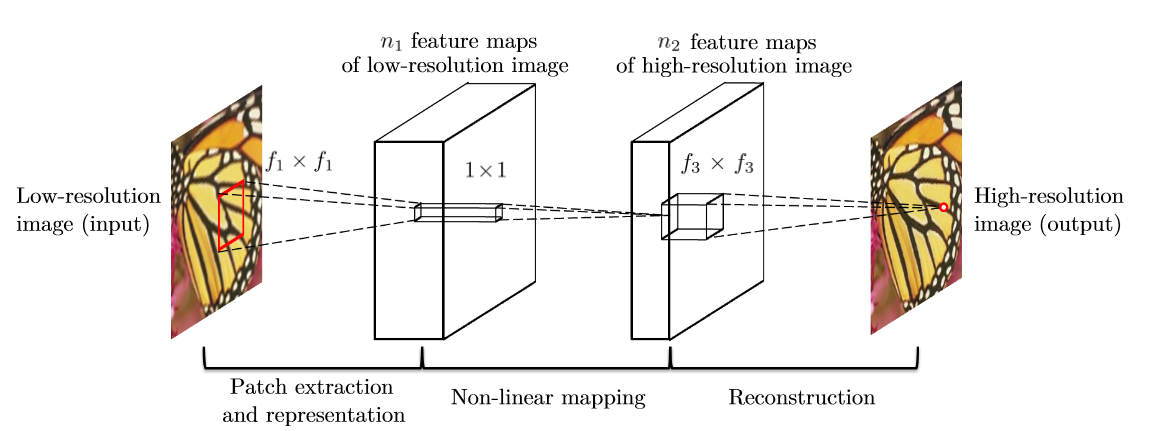
\includegraphics[width=1.0\textwidth]{imgs/SRCNN.png}
    \caption{SRCNN}
    \label{fig:SRCNN}
\end{figure}

\subsection{基于深度网络的图像超分辨率的改进方向}
% 这里主要介绍可改进的点

由于SRCNN较为简单,不能完全利用卷积神经网络的优势,故后人从多个方面对SRCNN进行了改进。

\subsubsection*{模型深度}
在VDSR中,Kim等人引入了更多的卷积层,从原来的3层增加到了20层,从而增强了网络的特征提取能力。由于卷积层数的增加势必带来计算量的增加,VDSR中使用了较小的卷积核($3\times3$),降低了模型的计算量。为了能够降低学习的难度,不同于SRCNN的直接学习高分辨率图像,VDSR学习的是高分辨率图像域双三次上采样图像之间的差值。网络结构为\ref{fig:VDSR}。在推理过程中,将双三次上采样图像与网络输出的差值相加即可得到超分辨率图像,用公式表达为

\begin{equation}
    y^r = y^b + \text{Convs}(y^b)
\end{equation}

\begin{figure}[htbp]
    \centering
    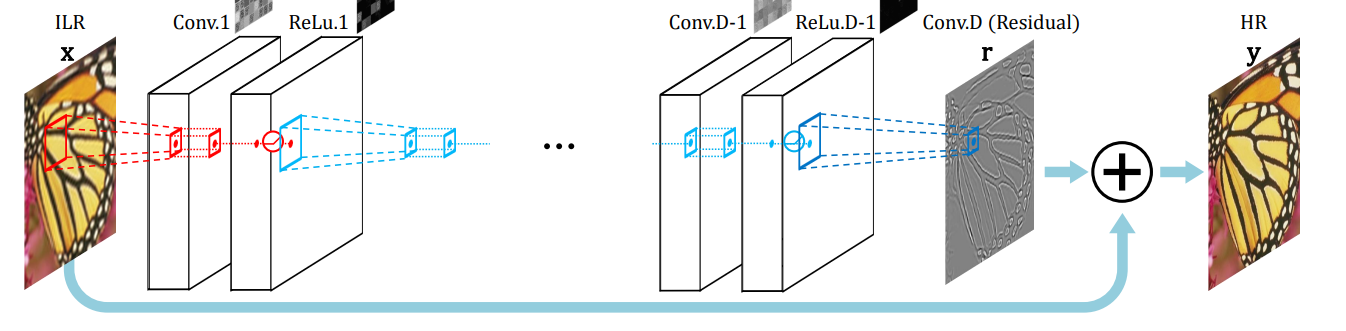
\includegraphics[width=1.0\textwidth]{imgs/VDSR.png}
    \caption{VDSR}
    \label{fig:VDSR}
\end{figure}

\subsubsection*{残差连接}
在计算机视觉其他领域的研究已经表明,过深的网络会带来不可避免的梯度爆炸或梯度消失问题。为了解决此问题,He等人提出了ResNet,通过残差连接使得梯度可以直接从深层网络传播到浅层网络,避免了梯度消失和梯度爆炸。在图像超分辨率中,也需要较深的网络来提取更强大的特征,故引入残差连接是有必要的。为此,Lim等人提出了EDSR,此模型中,作者引入了如图\ref{fig:EDSR—res}中所示的残差块:残差块的输入将分别经过一个卷积层、一个激活层和一个卷积层,并将结果与残差块的输入相加,得到残差块的输出,即$x_{l+1}=x_l+\text{Conv}(\text{Relu}(\text{Conv}(x_l)))$。网络由若干个相同的残差块组成。整体网络结构如图\ref{fig:EDSR},与此前模型的先上采样再重建图像的过程不同,EDSR先对LR图像进行处理,然后用不同的上采样头对特征进行上采样,以获得不同放大倍率的超分图像,提高了模型的泛化性,降低了训练的成本。


\begin{figure}[htbp]
    \subcaptionbox{\label{fig:EDSR—res}}{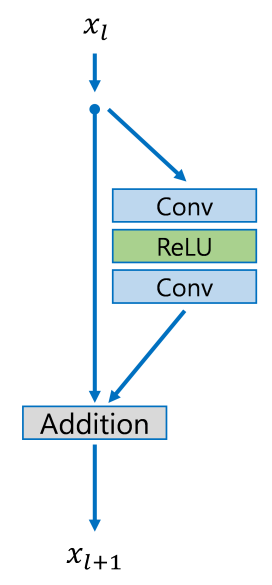
\includegraphics[width=.3\linewidth]{imgs/EDSR_res.png}}\hfill
    \subcaptionbox{\label{fig:EDSR}}{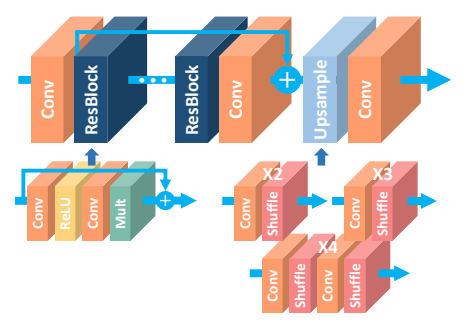
\includegraphics[width=.6\linewidth]{imgs/EDSR.png}}
    \caption{EDSR的结构:其中,图(a)为残差块的结构,图(b)为模型整体结构}	
    \label{fig:EDSR-struct}
\end{figure}


\subsubsection*{生成对抗网络}
Ledig等人提出的SRGAN结构如图\ref{fig:SRGAN}所示,其中,生成器(Generator)负责生成更为真实的高分辨率图像,而判别器(Discriminator)则负责分辨生成的高分辨率图像和真实数据集中的高分辨率图像。由于GAN模型较其他生成式模型来说具有生成更加逼真的图像的性质,通过这一框架,对大的放大倍率来说,可以重建出更为真实的高分辨率图像。此后,超分辨率模型多会基于GAN设计,本文亦是如此。


\begin{figure}[htbp]
    \centering
    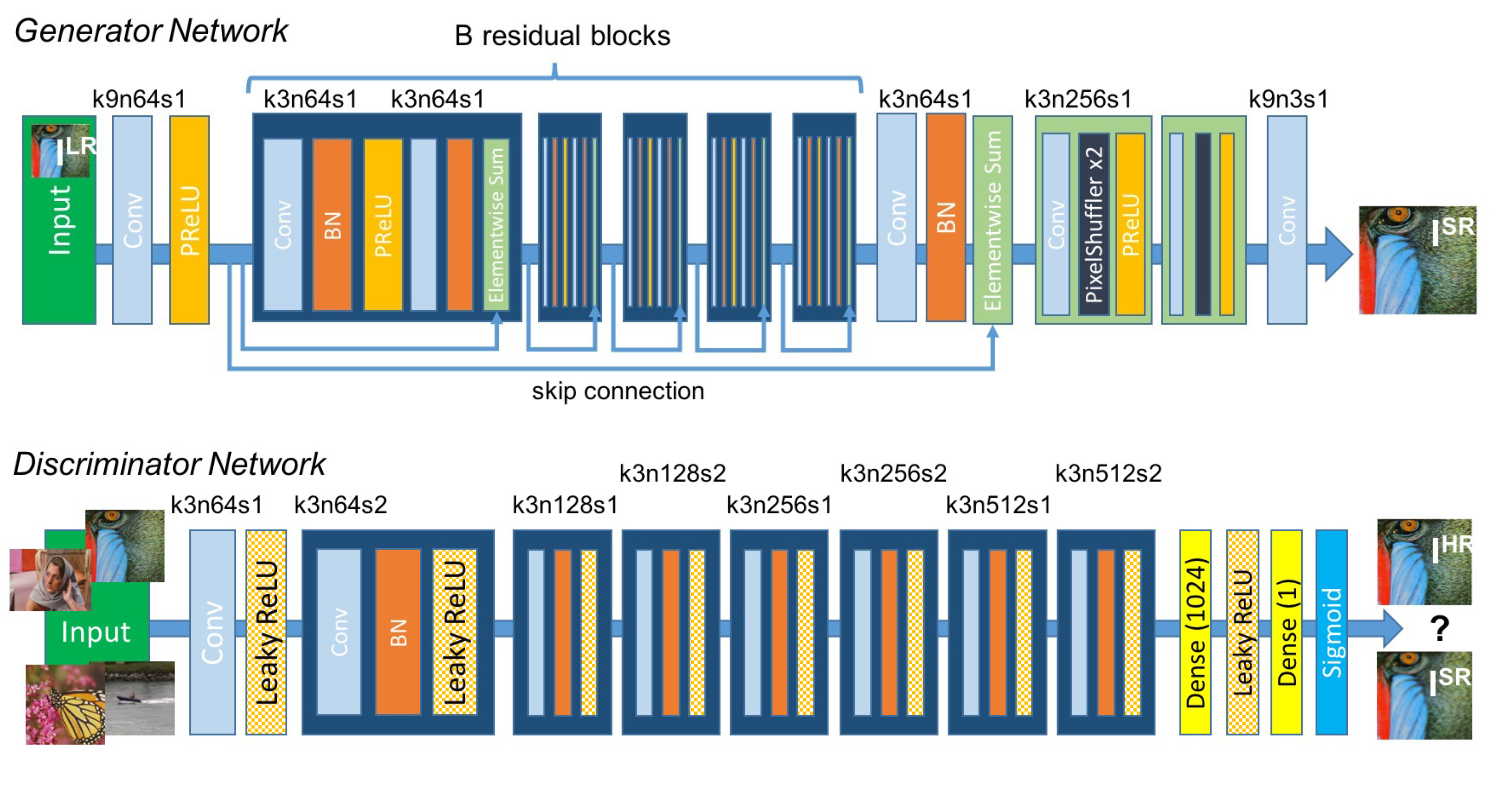
\includegraphics[width=0.8\textwidth]{imgs/SRGAN.png}
    \caption{SRGAN}
    \label{fig:SRGAN}
\end{figure}

\section{基于双三次下采样的低分辨率图像生成}
早期的超分辨率模型往往使用经过双三次下采样产生的合成数据集进行训练,其优点是数据集获取简单,运算量较小,速度较快。其公式描述为
\begin{equation}
    \mathbi{I}^{LR}=(\vb*{k}_g\otimes \mathbi{I}^{HR})\downarrow_s\label{equ:bicubic}
\end{equation}
其中$\vb*{k}_g$为高斯模糊核,$\otimes$表示卷积操作,$\mathbi{I}^{HR}$表示高分辨率图像,$\downarrow_s$表示双三次下采样。之所以先对高分辨率图像进行高斯滤波再下采样是因为根据奈奎斯特定理,当采样率小于等于信号频率的二倍时,将会造成失真,而对图像进行滤波则可以避免这种失真。对于双三次下采样,新图像中的每个像素点是由其在原图像中的位置周围$4\times4$共16个像素点的加权和计算而来的。对于如图\ref{fig:Bicubic}中的例子来说,新图像中的像素点对应为原图像中的$(i+u,j+v)$,其值为由$(i-1,j-1)$到$(i+2,j+2)$这16个像素的甲醛和计算。使用公式表述为
\begin{equation}
    \begin{split}
        &f(i+u,j+v)=ABC\\
        \text{其中}\\
        &A=
        \left[\begin{array}{c}
            S(1+v) \\
            S(v) \\
            S(1-v) \\
            S(2-v)
        \end{array}\right]^T\\
        &B=
        \left[\begin{array}{cccc}
            f(i-1,j-1) & f(i-1,j) & f(i-1,j+1) & f(i-1,j+2) \\
            f(i,j-1) & f(i,j) & f(i,j+1) & f(i,j+2) \\
            f(i+1,j-1) & f(i+1,j) & f(i+1,j+1) & f(i+1,j+2) \\
            f(i+2,j-1) & f(i+2,j) & f(i+2,j+1) & f(i+2,j+2)
        \end{array}\right]\\
        &C=
        \left[\begin{array}{c}
            S(1+u) \\
            S(u) \\
            S(1-u) \\
            S(2-u)
        \end{array}\right]
    \end{split}
\end{equation}
其中,$S(x)$为双三次样条函数,是$\frac{\sin(x)}{x}$的近似函数。其表达式为
\begin{equation}
    S(X)=
    \begin{cases}
        1-2|x|^2+|x|^3,&0<|x|<1\\
        4-8|x|+5|x|^2-|x|^3,&1\le|x|<2\\
        0,&|x|\ge2
    \end{cases}
\end{equation}

\begin{figure}[htbp]
    \centering
    \captionbox{双三次下采样示例\label{fig:Bicubic}}{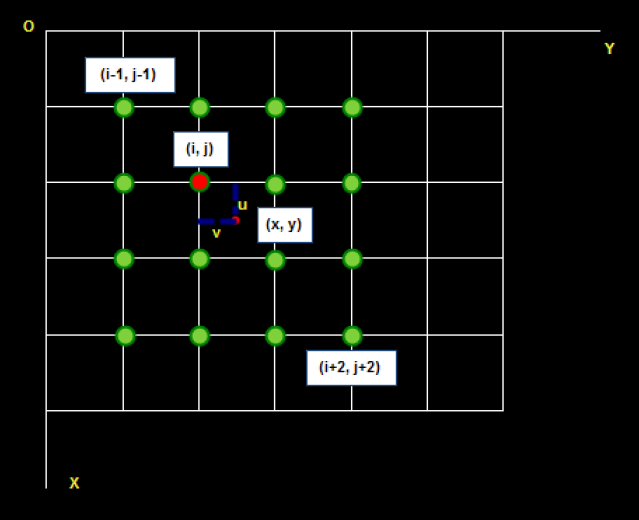
\includegraphics[width=.5\linewidth]{imgs/bicubic.png}}\hfill
    \captionbox{真实低分辨率图像的分布\label{fig:laplace}}{\includegraphics[width=.4\linewidth]{imgs/laplace.png}}
\end{figure} 


\section{真实低分辨率图像仿真生成方法}

真实低分辨率图像的仿真生成是无监督图像超分辨率模型中的重要一环。由于模型的超分辨率网络使用了生成的低分辨率图像进行训练,故生成图像与真实图像的贴近程度决定了超分辨率网络能否更好地学习到真实的低分辨率图像到高分辨率图像的重建方式。近年来,研究人员们提出了许多不同的仿真生成低分辨率图像的思路,形成了多种多样的模型。下面介绍一些经典的思路。

\subsection{高低频信息分离}
DSGAN\cite{fritsche2019frequency},全称DownSamplingGAN,是首先系统性地提出仿真生成低分辨率图像的方法的工作。模型的降采样部分如图\ref{fig:DSGAN-DSN}所示。首先将高分辨率图像进行双三次下采样,再使用网络进行后续的处理。为保证生成图像的拟真度和还原度,需要在利用内容和感知损失限制生成器的解空间的同时用对抗性损失引入非成对真实低分辨率图像的特征,而此前的研究中,二者的权衡很难做到,使得网络的学习变得困难。作者注意到,图像在降采样过程中,会丢失高频特征,而仅保留包含了颜色和上下文的低频特征,故模型要做到的就是学习真实图像的高频特征,而约束其低频特征与输入图像一致。作者通过高、低频高斯滤波器过滤出了低频特征用于计算内容损失$L_{col,d}$,而高频特征用于计算对抗性损失$L_{tex,d}$。通过此模型,可以针对只有高分辨率图像的数据集生成大量伪成对的低分辨率图像。

\subsection{域距离感知训练}
虽然对高低频信息的分离降低了学习的难度,但是仍然不能保证生成的图像与真实的图像在高频信息上保持一致,这样,二者之间就存在域距离。而域距离较大的图像对超分辨率模型的训练则可能带来负面的影响。故Wei等人\cite{Wei_2021_CVPR}提出了基于域距离感知训练的真实图像超分辨率模型DASR,解决了此问题。模型的DSN部分如图\ref{fig:DASR-DSN}所示,与DSGAN不同,DASR选用了小波变换来抽取高、低频信息,并且,在判别器部分,DASR使用了PatchGAN的策略,即针对生成图像中的每个图像块,都用判别器计算了与真实图像的相似性,从而形成了一个相似度矩阵$w$。在超分辨率网络\ref{fig:DASR-SRN}的内容损失和感知损失中,作者使用了L1损失,其中,对每张超分辨率图像与真实高分辨率图像的差,都按元素与相似度$w$相乘,从而使得图像中与真实图像域距离不同的区域对模型的优化有了不同的贡献,提高了模型学习的稳定性,让学习过程变得更为简单。

\begin{figure}[htbp]
    \subcaptionbox{\label{fig:DASR-DSN}}{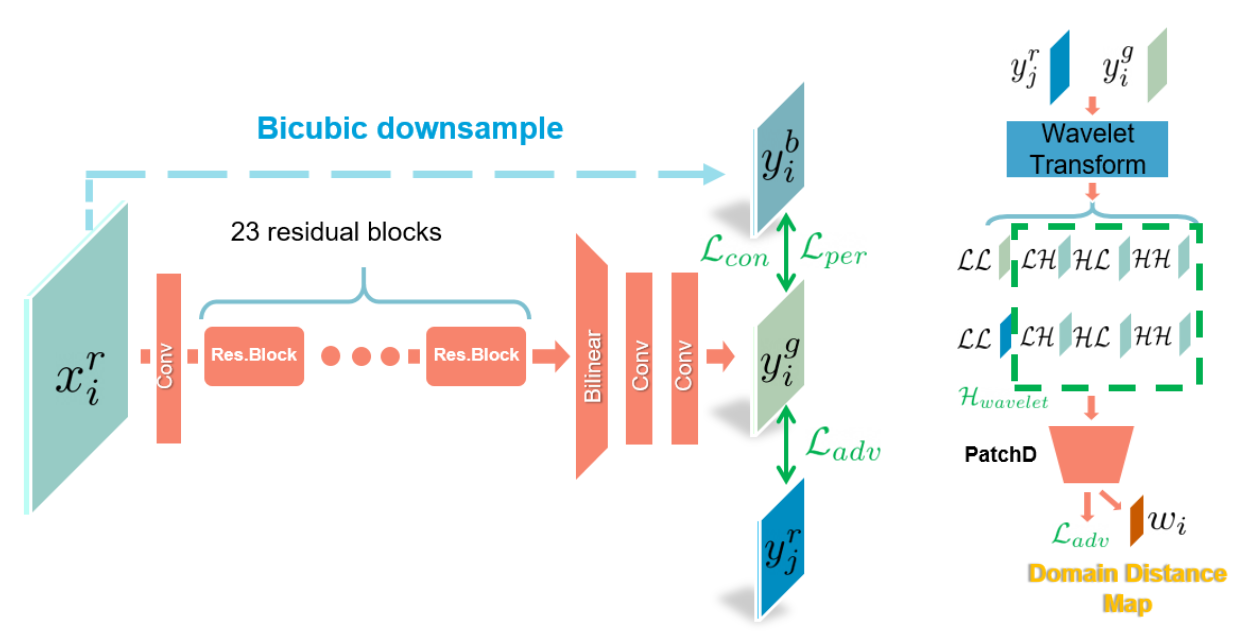
\includegraphics[width=.5\linewidth]{imgs/DASR-DSN.png}}\hfill
    \subcaptionbox{\label{fig:DASR-SRN}}{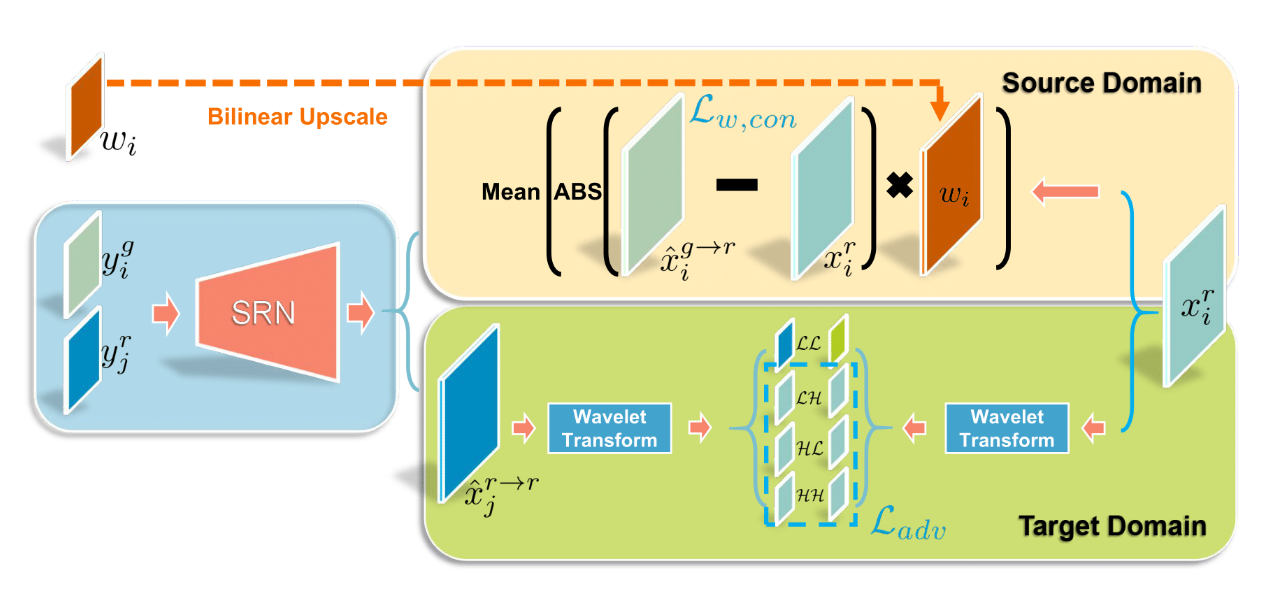
\includegraphics[width=.5\linewidth]{imgs/DASR-SRN.png}}
    \caption{DASR的结构:其中,图(a)为降采样网络(DSN),图(b)为超分辨率网络(SRN)}	
    \label{fig:DASR}
\end{figure}


\subsection{图像退化的不确定性}
在真实场景中,一张高分辨率图像往往可以经由不同的方式退化为多张不同但相似的低分辨率图像,而以往的模型对一张高分辨率图像往往只能生成一张对应的低分辨率图像。为了能够学习图像退化的不确定性,Ning等人\cite{ijcai2022p176}提出了基于退化不确定性学习的真实图像超分辨率模型USR-DU。作者首先探究了真实图像退化的不确定性规律,其实验结果如图\ref{fig:laplace}所示,其中横轴为像素差(0表示双三次下采样图像),纵轴为概率密度,图中直方图部分为收集到的数据,虚实两条曲线分别为拟合出的高斯分布和拉普拉斯分布。作者发现真实的低分辨率图像与双三次下采样图像之间的差异可以使用拉普拉斯分布来表征,而常用的高斯分布则不能很好地描述该不确定性。拉普拉斯分布的位置参数代表了低分辨率图像的基准像素值,而尺度参数则代表了像素值的不确定性。图\ref{fig:USR-DU-DSN}为DSN部分总体结构,DSN输入高分辨率图像,生成拟真的低分辨率图像$y_g$及其不确定性$\theta$,二者拥有相同的尺寸。生成的低分辨率图像与高分辨率图像的双三次下采样$y_b$结果计算内容损失,与非成对的真实低分辨率图像$y_r$计算对抗性损失。为了确保生成图像及其不确定性也满足拉普拉斯分布,在计算内容损失时,采用KL散度使得生成的分布逼近实际的分布(KL散度描述了估计分布与真实分布的相似度,KL散度的值越低,说明二者越相似),可描述为式\ref{equ:kl}。为了能在特征域也考虑不确定性,DSN另外生成了拟真低分辨率图像经由VGG\cite{simonyan2014very}提取的特征图的不确定性$\sigma$,并使用生成图像的特征图与双三次下采样图像的特征图计算感知损失(同样使用KL散度)。此外,如同\cite{fritsche2019frequency},作者在计算损失函数前,对图像分别进行了梯度计算处理与高斯高频滤波处理,分离了高低频信息。在DSN网络训练完成后,使用DSN并生成大量的伪成对数据集训练SRN。其中,伪成对数据集中的低分辨率图像由生成的低分辨率图像及其不确定性依照拉普拉斯分布随机采样获取。借由不确定性学习,USR-DU在减少伪影的同时提高了超分辨率图像的清晰度。



\begin{equation}
    \begin{aligned}
        \mathcal{L}_{kl}&=\mathbb{E}_{\vb*{y}_g}\{D_{\text{KL}}[L(\vb*{y}_g,\bm{\theta})\|L(\vb*{y}_b,\mathbi{I})]\}  \\
        &=\mathbb{E}_{\vb*{y}_g}[\bm{\theta}\exp(-\frac{\|\vb*{y}_g-\vb*{y}_b\|_1}{\bm{\theta}})+\|\vb*{y}_g-\vb*{y}_b\|_1-\ln\bm{\theta}-1]
    \end{aligned}
    \label{equ:kl}
\end{equation}








% \section{超分辨率模型的数据集}
% \subsection{常用的Benchmark数据集}
% 许多超分辨率模型会使用Set5\cite{Set5}、Set14\cite{Set14}等作为测试数据集(二者分别由5张图像和14张图像构成,其名称正是来自于此),用于与其他方法进行比较。以上数据集只提供高分辨率图像,而低分辨率图像通过双三次下采样产生,故经常用来评价基于合成图像的超分辨率模型。

% \subsection{真实图像超分辨率模型的数据集}
% 部分数据集同时提供了高分辨率图像和低分辨率图像,其中有些数据集的低分辨率图像由图像压缩和随机噪音产生,如DIV2K\cite{Agustsson_2017_CVPR_Workshops}和Flickr2K\cite{timofte2017ntire},其中,DIV2K包含800对成对的训练集图像和100对成对的验证集图像,Flickr2K作为NTIRE2017-2018比赛用数据集,拥有2650对成对的验证集图像。而另一些数据集通过调整相机焦距而取得了不同分辨率的图像,RealSR\cite{cai2019toward}是其中的代表,其包含Nikon和Canon两种相机拍摄的图像,二者均包含200对成对的训练集图像和50对成对的测试集图像,且分别提供2倍、3倍、4倍缩放的低分辨率图像。特别地,DPEDiphone\cite{ignatov2017dslr}数据集中仅包含由iphone3手机拍摄的5902张训练集图像和113张验证集图像,未提供对应的高分辨率图像。